\documentclass[12pt,a4paper]{article}
\usepackage{mathced}
\usepackage{caption}
\usepackage{graphicx}
\usepackage{xcolor}
\usepackage{listings}
\usepackage[left=2.5cm,right=2.5cm,top=3cm,bottom=2cm]{geometry}

\usepackage[hyperref=true,backend=bibtex,citestyle=alphabetic,bibstyle=ieee,style=alphabetic,backref=true]{biblatex}
\bibliography{bibli.bib}

\definecolor{dkgreen}{rgb}{0,0.6,0}
\definecolor{gray}{rgb}{0.5,0.5,0.5}
\definecolor{mauve}{rgb}{0.58,0,0.82}
\definecolor{redW}{rgb}{1,0.5,0.3}

\lstset{frame=tb,
  aboveskip=1mm,
  belowskip=1mm,
  showstringspaces=false,
  columns=flexible,
  basicstyle={\footnotesize\ttfamily},
  numbers=none,
  numberstyle=\tiny\color{gray},
  keywordstyle=\color{blue},
  commentstyle=\color{dkgreen},
  stringstyle=\color{mauve},
  breaklines=true,
  breakatwhitespace=true,
  tabsize=2
}

\lstdefinelanguage{plm}
{
keywordstyle=[2]
morekeywords={interface, Vlan, line, ip, hostname, no},
sensitive=false,
morecomment=[l]{!},
morecomment=[s]{/*}{*/},
%morestring=[b]",
%classoffset=0,
%morekeywords={standby},keywordstyle=\color{redW},
classoffset=1,
morekeywords={os, plm_version, evt_type, java_version, start_date, course, exolang, exoswitchto, totaltests, passedtests, exoname, username,lastUsed,userUUID},keywordstyle=\color{blue},
classoffset=0
}

\usepackage{tikz}
\usetikzlibrary{backgrounds,calc,shadings,shapes.arrows,shapes.symbols,shadows}
\tikzset{every picture/.style={execute at begin picture={
   \shorthandoff{:;!?};}
}}

\definecolor{switch}{HTML}{006996}
\definecolor{filtrage}{HTML}{FF7066}

\makeatletter
\pgfkeys{/pgf/.cd,
  parallelepiped offset x/.initial=2mm,
  parallelepiped offset y/.initial=2mm
}
\pgfdeclareshape{parallelepiped}
{
  \inheritsavedanchors[from=rectangle] % this is nearly a rectangle
  \inheritanchorborder[from=rectangle]
  \inheritanchor[from=rectangle]{north}
  \inheritanchor[from=rectangle]{north west}
  \inheritanchor[from=rectangle]{north east}
  \inheritanchor[from=rectangle]{center}
  \inheritanchor[from=rectangle]{west}
  \inheritanchor[from=rectangle]{east}
  \inheritanchor[from=rectangle]{mid}
  \inheritanchor[from=rectangle]{mid west}
  \inheritanchor[from=rectangle]{mid east}
  \inheritanchor[from=rectangle]{base}
  \inheritanchor[from=rectangle]{base west}
  \inheritanchor[from=rectangle]{base east}
  \inheritanchor[from=rectangle]{south}
  \inheritanchor[from=rectangle]{south west}
  \inheritanchor[from=rectangle]{south east}
  \backgroundpath{
    % store lower right in xa/ya and upper right in xb/yb
    \southwest \pgf@xa=\pgf@x \pgf@ya=\pgf@y
    \northeast \pgf@xb=\pgf@x \pgf@yb=\pgf@y
    \pgfmathsetlength\pgfutil@tempdima{\pgfkeysvalueof{/pgf/parallelepiped
      offset x}}
    \pgfmathsetlength\pgfutil@tempdimb{\pgfkeysvalueof{/pgf/parallelepiped
      offset y}}
    \def\ppd@offset{\pgfpoint{\pgfutil@tempdima}{\pgfutil@tempdimb}}
    \pgfpathmoveto{\pgfqpoint{\pgf@xa}{\pgf@ya}}
    \pgfpathlineto{\pgfqpoint{\pgf@xb}{\pgf@ya}}
    \pgfpathlineto{\pgfqpoint{\pgf@xb}{\pgf@yb}}
    \pgfpathlineto{\pgfqpoint{\pgf@xa}{\pgf@yb}}
    \pgfpathclose
    \pgfpathmoveto{\pgfqpoint{\pgf@xb}{\pgf@ya}}
    \pgfpathlineto{\pgfpointadd{\pgfpoint{\pgf@xb}{\pgf@ya}}{\ppd@offset}}
    \pgfpathlineto{\pgfpointadd{\pgfpoint{\pgf@xb}{\pgf@yb}}{\ppd@offset}}
    \pgfpathlineto{\pgfpointadd{\pgfpoint{\pgf@xa}{\pgf@yb}}{\ppd@offset}}
    \pgfpathlineto{\pgfqpoint{\pgf@xa}{\pgf@yb}}
    \pgfpathmoveto{\pgfqpoint{\pgf@xb}{\pgf@yb}}
    \pgfpathlineto{\pgfpointadd{\pgfpoint{\pgf@xb}{\pgf@yb}}{\ppd@offset}}
  }
}
\makeatother

\tikzset{
  ports/.style={
    line width=0.3pt,
    top color=gray!20,
    bottom color=gray!80
  },
  server/.style={
    parallelepiped,
    fill=white, draw,
    minimum width=0.35cm,
    minimum height=0.75cm,
    parallelepiped offset x=3mm,
    parallelepiped offset y=2mm,
    xscale=-1,
    path picture={
      \draw[top color=gray!5,bottom color=gray!40]
      (path picture bounding box.south west) rectangle 
      (path picture bounding box.north east);
      \coordinate (A-center) at ($(path picture bounding box.center)!0!(path
        picture bounding box.south)$);
      \coordinate (A-west) at ([xshift=-0.575cm]path picture bounding box.west);
      \draw[ports]([yshift=0.1cm]$(A-west)!0!(A-center)$)
        rectangle +(0.2,0.065);
      \draw[ports]([yshift=0.01cm]$(A-west)!0.085!(A-center)$)
        rectangle +(0.15,0.05);
      \fill[black]([yshift=-0.35cm]$(A-west)!-0.1!(A-center)$)
        rectangle +(0.235,0.0175);
      \fill[black]([yshift=-0.385cm]$(A-west)!-0.1!(A-center)$)
        rectangle +(0.235,0.0175);
      \fill[black]([yshift=-0.42cm]$(A-west)!-0.1!(A-center)$)
        rectangle +(0.235,0.0175);
    }  
  },
}

\usetikzlibrary{calc, shadings, shadows, shapes.arrows}

% Styles for interfaces and edge labels
\tikzset{%
  interface/.style={draw, rectangle, rounded corners, font=\LARGE\sffamily},
  ethernet/.style={interface, fill=yellow!50},% ethernet interface
  serial/.style={interface, fill=green!70},% serial interface
  speed/.style={sloped, anchor=south, font=\large\sffamily},% line speed at edge
  route/.style={draw, shape=single arrow, single arrow head extend=4mm,
    minimum height=1.7cm, minimum width=3mm, white, fill=switch!20,
    drop shadow={opacity=.8, fill=switch}, font=\tiny}% inroute/outroute arrows
}
\newcommand*{\shift}{1.3cm}% For placing the arrows later

% The router icon
\newcommand*{\router}[1]{
\begin{tikzpicture}    
  \coordinate (ll) at (-3,0.5);
  \coordinate (lr) at (3,0.5);
  \coordinate (ul) at (-3,2);
  \coordinate (ur) at (3,2);
  \shade [shading angle=90, left color=switch, right color=white] (ll)
    arc (-180:-60:3cm and .75cm) -- +(0,1.5) arc (-60:-180:3cm and .75cm)
    -- cycle;
  \shade [shading angle=270, right color=switch, left color=white!50] (lr)
    arc (0:-60:3cm and .75cm) -- +(0,1.5) arc (-60:0:3cm and .75cm) -- cycle;
  \draw [thick] (ll) arc (-180:0:3cm and .75cm)
    -- (ur) arc (0:-180:3cm and .75cm) -- cycle;
  \draw [thick, shade, upper left=switch, lower left=switch,
    upper right=switch, lower right=white] (ul)
    arc (-180:180:3cm and .75cm);
  \node at (0,0.5){\color{blue!60!black}\Huge #1};% The name of the router
  % The four arrows, symbols for incoming and outgoing routes:
  \begin{scope}[yshift=2cm, yscale=0.28, transform shape]
    \node[route, rotate=45, xshift=\shift] {\strut};
    \node[route, rotate=-45, xshift=-\shift] {\strut};
    \node[route, rotate=-135, xshift=\shift] {\strut};
    \node[route, rotate=135, xshift=-\shift] {\strut};
  \end{scope}
\end{tikzpicture}}

\makeatletter
\pgfdeclareradialshading[tikz@ball]{cloud}{\pgfpoint{-0.275cm}{0.4cm}}{%
  color(0cm)=(tikz@ball!75!white);
  color(0.1cm)=(tikz@ball!85!white); 
  color(0.2cm)=(tikz@ball!95!white); 
  color(0.7cm)=(tikz@ball!89!black); 
  color(1cm)=(tikz@ball!75!black)
}
\tikzoption{cloud color}{\pgfutil@colorlet{tikz@ball}{#1}%
  \def\tikz@shading{cloud}\tikz@addmode{\tikz@mode@shadetrue}}
\makeatother

\tikzset{my cloud/.style={
     cloud, draw, aspect=2,
     cloud color={gray!5!white}
  }
}


\author{Mathieu Morainville et Cédric Huguenin}
\title{Rapport PIDR}
\newcommand{\reporttitle}{Serveur d'application pour la Programmer's Learning Machine}     % Titre
\newcommand{\reportauthor}{Mathieu \textsc{Morainville} \\ \& Cédric \textsc{Huguenin}} % Auteurs
\newcommand{\reportresponsables}{Martin \textsc{Quinson} \\ \& Gérald \textsc{Oster}} % Responsables
\newcommand{\reportsubject}{Projet Interdisciplinaire ou Découverte de la Recherche} % Sujet
\newcommand{\HRule}{\rule{\linewidth}{0.5mm}}
\setlength{\parskip}{1ex} % Espace entre les paragraphes

\begin{document}
  \begin{titlepage}
$ $\\$ $\\$ $\\$ $\\
\begin{center}

\begin{minipage}[t]{0.48\textwidth}
  \begin{flushleft}
    
\includegraphics [width=50mm]{images/TN.eps} \\[0.5cm]
      \textsc{\LARGE TELECOM Nancy \\}{\small 193 av. Paul Muller\\54602 Villers-Lès-Nancy}
  \end{flushleft}
\end{minipage}
\begin{minipage}[t]{0.48\textwidth}
  \begin{flushright}
    
\includegraphics [width=50mm]{images/loria.eps} \\[0.5cm]
    \textsc{\LARGE LORIA\\}{\small Campus scientifique\\BP 239\\54506 Vandoeuvre-lès-Nancy Cedex}
  \end{flushright}
\end{minipage} \\[1.5cm]

\textsc{\Large \reportsubject}\\[0.5cm]
\HRule \\[0.7cm]
{\Huge \bfseries \reporttitle}\\[0.4cm]
\HRule \\[1.5cm]

\begin{minipage}[t]{0.3\textwidth}
  \begin{flushleft} \large
    \emph{Auteurs :}\\
    \reportauthor
  \end{flushleft}
\end{minipage}
\begin{minipage}[t]{0.6\textwidth}
  \begin{flushright} \large
    \emph{Responsables :} \\
    \reportresponsables
  \end{flushright}
\end{minipage}

\vfill

{\large TELECOM Nancy deuxième année (2013-2014)}

\end{center}

\end{titlepage}

  \cleardoublepage % Dans le cas du recto verso, ajoute une page blanche si besoin
  \sloppy          % Justification moins stricte : des mots ne dépasseront pas des paragraphes
  \cleardoublepage
\section*{Remerciements}
  \addcontentsline{toc}{section}{Remerciements}

Nous tenons à remercier Messieurs Martin Quinson et Gérald Oster pour leur soutien et leur disponibilité tout au long du projet ainsi que pour leur enthousiasme et les échanges d'idées intéressants que nous avons pu avoir lors des réunions.
\bigskip \bigskip \bigskip

%\section*{Avant-propos} % Pas de numérotation
%\addcontentsline{toc}{section}{Avant-propos} % Ajout dans la table des matières
  
  \tableofcontents % Table des matières
  \cleardoublepage

\section{Introduction}
	La Programmer's Learning Machine\cite{PLMQuinson} est une plate-forme d'enseignement de la programmation développée par Gérald Oster et Martin Quinson dans le cadre des cours à Telecom Nancy depuis 2007. Depuis sa création, l'outil a été utilisé dans le module de remise a niveau en informatique proposé aux élèves venant des CPGE en début de première année ainsi que dans le module \og techniques et outils pour programmer\fg{}. Cette plate-forme présente plusieurs avantages pédagogiques. Tout d'abord, elle permet la mise en œuvre pratique des notions abordées en cours de façon théorique et parfois déroutante pour les débutants. Ensuite, la représentation graphique des problèmes semble plus motivante pour les étudiants. De plus, l'exécution interactive et son cycle de développement/tests court permet aux étudiants d'évaluer eux-mêmes leur travail et de résoudre les problèmes de façon incrémentale. Enfin, la base relativement importantes d'exercices permet à chacun de s'entraîner individuellement à son rythme jusqu'à maîtriser les notions abordées. Dans son état actuel, l'environnement est surtout centré sur l'élève : il reste difficile pour l'enseignant de suivre les avancées des élèves pendant la séance afin de détecter les élèves ayant besoin d'aide, c'est-à-dire ceux qui sont bloqués sur un exercice.

C'est dans ce contexte que se situe notre PIDR (Projet Interdisciplinaire ou Découverte de la Recherche). Ce projet encadré par un enseignant-chercheur ou un chercheur permet un premier contact concret avec la recherche menée dans les laboratoires de l'Université, en particulier le LORIA, le CRAN et l'IECN. Dans le cas interdisciplinaire, le projet ne se déroule pas nécessairement en laboratoire et concerne des aspects liés à différentes disciplines autour de l'informatique. Dans notre cas, il s'agit des aspects pédagogiques liés à l'apprentissage de la programmation. Durant les quatre mois pendant lesquels se déroule le PIDR, nous devrons donc trouver et mettre en œuvre des solutions pour qu'il soit plus facile pour les enseignants comme pour les élèves de suivre les progrès réalisés lors de la résolution des exercices.


%* Préciser le contexte du problème : qui est concerné ? Dans quel cadre spatial et temporel ?

%* En quoi la situation actuelle est-elle insatisfaisante ? Quelle(s) amélioration(s) faudrait-il apporter ?

%* Quels sont les enjeux ?
\newpage
\section{Analyse du problème}
Tout d'abord, nous allons dans cette première partie présenter l'état de la PLM au début du projet puis analyser les problèmes à traiter pour faire en sorte qu'elle réponde aux besoins du sujet. Nous énoncerons alors plus clairement le but à atteindre et décrirons les améliorations à apporter afin de remplir les objectifs poursuivis.

\subsection{Situation de départ}

La PLM existe depuis 2007 et se trouve donc dans un stade de développement très avancé, ayant également été amélioré au travers d'autres PIDR. Le nombre élevé de classes et de packages la composant nécessite donc de la modifier avec soin et de s'assurer que chaque modification n'entrave pas son fonctionnement. Pour cela des tests unitaires concernant les exercices existent (\texttt{plm.core}, fichier ExoTest.java) et nous devions nous assurer qu'après chaque modification importante nous pouvions encore passer chacun de ces tests.


Au départ, et comme nous l'avons stipulé dans l'introduction, la PLM est déjà un outil pédagogique très utile pour les élèves. Néanmoins, à ce moment, ces derniers ne pouvaient récupérer leur ancien code que s'ils se connectaient sur la même session que celle sur laquelle ils avaient ouvert la PLM pour la dernière fois. Ceci afin de pouvoir récupérer les données stockées dans le répertoire .plm, qui stocke sous forme de fichiers zip diverses informations sur l'avancement de l'utilisateur en question et notamment le code source de chaque exercice qu'il a tenté et/ou réussi. Le classe qui s'occupe d'enregistrer et de charger le code source de l'élève s'appelle ZipSessionKit, du package \texttt{plm.core.model.session}.


Cette classe n'est cependant pas très adaptée à une utilisation de la PLM en mode \og connecté\fg{} pour ainsi dire. En effet, la compression opérée sur les fichiers ne permet pas un traitement aisée des données. Ainsi pour l'instant, l'utilisateur n'a aucun moyen de récupérer son code sur une autre machine autre que celui de copier son répertoire .plm sur une clé et de le coller au bon endroit sur un autre ordinateur.


Avec la volonté de déporter les données des utilisateurs vers un serveur pour y avoir accès plus facilement, d'autres questions se sont posées et, pour résumer également ce qui a été dit précédemment, les problèmes suivants ont été remarqués :
\begin{itemize}
\item l'utilisateur n'a pas de moyen simple de retrouver son avancement sur une autre machine ;
\item l'utilisateur et les professeurs n'ont pas de moyen simple de consulter les résultats des exercices réalisés ;
\item l'historique des modifications n'est pas sauvegardé ;
\item il y a un seulement un utilisateur par machine.
\end{itemize}

\subsection{But à atteindre}


À terme, la PLM devrait pouvoir être utilisé efficacement non seulement par les élèves mais également les professeurs, qui pourront avoir accès aux données des élèves via une interface d'administration sur un serveur distant afin d'en tirer éventuellement des statistiques ou des conclusions quant au travail effectué par les élèves. Cela leur permettrait alors d'être plus efficace lors des séances de travail PLM et de pouvoir adapter leurs objectifs d'enseignement.


Afin de déporter les données générées par la PLM et de permettre son utilisation sur différentes machines,  les améliorations suivantes seront à traiter :

\begin{itemize}
\item les modifications d'un utilisateur sont stockés à la fois localement mais aussi sur un serveur distant ;
\item dès lors que les données d'un utilisateur sont stockées \og dans le nuage\fg{}, les progrès de cet élève sont consultables à distance via une interface web par les professeurs ;
\item l'utilisateur devrait être en mesure de pouvoir récupérer sa progression sur n'importe quel machine ;
\item il pourrait alors être intéressant de gérer plusieurs utilisateurs sur une même machine et de permettre de passer de l'un à l'autre facilement.
\end{itemize}


\subsection{Problèmes rencontrés}

Lors de l'analyse du problème et de la recherche de solutions pour mener à bien notre projet, plusieurs problèmes se sont posés. Cette partie va nous servir à faire le point sur ces différentes difficultés et à les expliquer plus en détail.

\subsubsection[ZipSessionKit]{ZipSessionKit \hyperref[zipSessionSol]{$\downarrow$}}
\label{zipSessionPb}

La PLM actuelle propose une interface ISessionKit qui doit être implémentée par les objets dont la responsabilité est de stocker le code de l'utilisateur sur le disque mais aussi de le charger pour qu'il puisse continuer son travail. En plus, il doit renseigner la PLM sur les exercices déjà réussis en fonction des langages de programmation disponible.

L'objet qui est actuellement utilisé est ZipSessionKit. Comme son nom l'indique, il sauvegarde toutes les données utiles dans des archives zip : une par leçon. Chaque archive contient un dossier par langage et ces dossiers contiennent chacun autant de dossiers qu'il y a d'exercices dans la leçon.

Cette solution de stockage ne permet pas d'être facilement lue. Ainsi, elle ne convient pas à notre démarche d'extraction de données des travaux des élèves. De plus, elle ne donne que la dernière version du code de l'utilisateur. Nous aurions aimé profiter de la possibilité de changer cette façon de stocker les sessions des utilisateurs pour mettre en place un système qui conserverait toutes les étapes du code de l'utilisateur.

\subsubsection[Serveur distant]{Serveur distant \hyperref[serveurDistantSol]{$\downarrow$}}
\label{serveurDistantPb}

En imaginant avoir un objet implémentant l'interface ISessionKit d'une façon qui permette de remplir nos objectifs plus simplement, le code de l'élève resterait pour le moment toujours sur sa machine locale. Le but de notre projet étant de pouvoir récupérer le code de tous les utilisateurs de la PLM qui sont connectés à Internet, il faudrait donc que l'implémentation d'ISessionKit permette d'envoyer le code sur un serveur distant.

\subsubsection[Anonymat des données]{Anonymat des données \hyperref[anonymatSol]{$\downarrow$}}
\label{anonymatPb}

L'anonymat des données est primordial. Les utilisateurs avertis se méfient de plus en plus du respect de la vie privée dans le monde numérique. Les données recueillies doivent être accessible au plus grand nombre sans permettre d'identifier les utilisateurs. En effet, les données pourront alors servir aux chercheurs et aux professeurs.

\subsubsection[Identification des utilisateurs]{Identification des utilisateurs \hyperref[identifSol]{$\downarrow$}}
\label{identifPb}

En apparente contradiction directe avec le problème précédent, il est à noter que comme les données doivent aussi permettre aux professeurs de suivre le travail de leurs élèves, il est impératif d'avoir un système capable de lier une identité sur un utilisateur anonyme. Ce système serait indépendant de l'implémentation du ISessionKit utilisé. Le système doit aussi être simple pour les utilisateurs : il devrait, dans l'idéal, ne pas nécessiter de mot de passe mais tout de même permettre une certaine sécurité. Ce système ne sera utilisé que dans le cadre éducatif a priori et donc seuls les professeurs pourront effectivement faire le lien entre une identité anonyme et un élève en particulier.



%Montrer précisément la différence entre la situation actuelle et le but à atteindre.
%
%* Connaissance des causes de la situation insatisfaisante
%
%* Description des améliorations à apporter et des objectifs poursuivis (ex. : gain de temps, d'argent, etc.) : cahier des charges du projet.
\newpage
\section{Organisation}

Après avoir analysé l'état de la PLM au début du projet, nous devions nous organiser, aussi bien avec nos encadrants qu'entre nous, pour pouvoir mener à bien notre PIDR. Cette partie a donc pour but de décrire notre méthode de travail et la façon dont nous nous sommes réparti les tâches au cours des quatre mois du projet.

\subsection{Méthode de travail}

Au commencement du projet, nous avons convenu avec Martin Quinson et Gérald Oster de nous réunir chaque mercredi afin de faire le point sur les progrès réalisés mais également et surtout de définir les limites et le cadre du projet. En effet, beaucoup d'améliorations peuvent encore être apportées à la PLM et les premières réunions étaient surtout des brainstormings afin de trouver des idées et de voir ce qui pouvait être fait dans le cadre temporel limité du PIDR.


\`A la fin de chaque réunion, nous nous fixions une liste de choses à faire pour la prochaine réunion et entre chaque réunion nous nous efforcions donc de mener à bien ces tâches. Lorsque les limites du projet étaient mieux définies et que les tâches à effectuer commençaient à devenir plus complexes, les fréquences des réunions se sont espacées afin de toujours nous permettre de mener à bien nos tâches. Lorsque les réunions ne pouvaient vraiment pas avoir lieues pour cause d'indisponibilités ou d'incompatibilité des emplois de temps, nous envoyions tout de même un mail récapitulatif quand l'avancement nous semblait assez significatif.


Pour nous permettre de prendre facilement part au développement de la PLM, nous avons également forké le dépôt GitHub de la PLM\cite{OsterGitHub} afin de pouvoir faire des pulls requests dès que nous avions des modifications stables à incorporer à la PLM.


\subsection{Comptes-rendus des réunions}

Afin de mieux se rendre de l'évolution des attentes et des tâches à réaliser au fur et à mesure de l'évolution du temps, nous avons décidé d'écrire dans cette section les résumés des principales réunions que nous avons eues avec nos encadrants.

\begin{description}
\item[15/01/2014] : $ $
	\begin{description}
	\item[Ordre du jour] : présentation du contexte, de la PLM et des attentes vis-à-vis du PIDR.
	\item[Décisions prises] : utiliser Git pour stocker les données des utilisateurs. Cela permettra de ne pas dépendre d'une technologie en particulier pour accéder à ces données.
	\item[\`A faire pour la prochaine réunion] : protocole sur papier, s'informer sur JGit, étudier le code de la PLM, notamment la partie sur les espions (\texttt{plm.core.model.tracking}).
	\end{description}
\end{description}

\begin{description}
\item[24/01/2014] : $ $
	\begin{description}
	\item[Ordre du jour] : présentation des buts à long terme de la PLM. Cadrage des limites du projet et des objectifs à court terme attendus.
	\item[Décisions prises] : ne pas essayer de tout faire, mais créer une base stable qui pourra être réutilisée ultérieurement.
	\item[À faire] : créer un espion Git qui commit localement.
	\end{description}
\end{description}

\begin{description}
\item[31/01/2014] $ $
	\begin{description}
	\item[Ordre du jour] : aller dans les détails et voir techniquement ce qu'il est possible de faire avec les outils à disposition.
	\item[Décisions prises] : écrire des Use Cases pour voir quelles implémentations et solutions sont envisageables en pratique.
	\item[À faire] : écrire les Use Cases, améliorer l'espion Git, se familiariser avec le framework Play.
	\end{description}
\end{description}

\begin{description}
\item[17/02/2014] $ $
	\begin{description}
	\item[Ordre du jour] : étudier les Use Cases.
	\item[Décisions prises] : demander le moins d'informations à l'utilisateur au démarrage de la PLM (éviter les mots de passe et les authentifications). Faire un lien entre une identité anonyme et un utilisateur.
	\item[À faire] : $ $
		\begin{itemize}
		\item - trouver un moyen de pusher anonymement avec JGit tout en permettant aux professeurs de trouver l'identité d'un élève derrière un commit anonyme ;
		\item simplifier les Use Cases ;
		\item  faire les premiers essais de push vers un dépôt Git distant avec JGit.
		\end{itemize}
	\end{description}
\end{description}

\begin{description}
\item[26/03/2014] $ $
	\begin{description}
	\item[Ordre du jour] : évaluation de l'état d'avancement et des solutions concrètes proposées.
	\item[Décisions prises] : rédaction des Use Cases/scénarios définitifs. Les utilisateurs seront identifiés par un identifiant unique.
	\item[À faire] : $ $
		\begin{itemize}
		\item - implémenter GitSessionKit pour remplacer ZipSessionKit ;
		\item faire en sorte que l'espion Git enregistre les changements aussi lorsqu'un utilisateur change d'exercice à l'intérieur de la PLM ;
		\item implémenter les différents scénarios.
		\end{itemize}
	\end{description}
\end{description}

\subsection{Tâches et répartition du travail}

Notre cheminement pour résoudre les différents problèmes posés au cours des réunions a connu plusieurs étapes. Nous nous sommes réparti les tâches selon la nature et la complexité de ces étapes et avons souvent dû réfléchir et programmer ensemble. Dans cette partie, nous allons donc présenter ces étapes d'une manière claire et simplifiée.

\begin{description}
\item[Première étape (5h)] : arriver à faire compiler correctement la PLM sur nos machines.

Pour compiler sous Eclipse, nous ne devions pas oublier d'installer le plugin Scala (\url{http://scala-ide.org/download/current.html}) et le plugin Python (\url{http://pydev.org/download.html}) et de bien configurer le Build Path.

\item[Deuxième étape (20 h)] : prendre connaissance du code et de la structure de la PLM.

Lors de cette étape, nous avons découvert un certain nombre de petits bugs que nous avons pu corriger et nous avons alors soumis la correction par Pull Requests. Ces bugs incluaient :

	\begin{itemize}
	\item correction des numéros de ligne affichés sous Windows lors d'une exception générée par le code d'un utilisateur ;
	\item encryption SSL des messages automatiques de succès postés sur Twitter ;
	\item correction d'un problème de synchronisation entre la vue utilisateur dans la PLM et le code sur le disque du à une frappe au clavier trop rapide ;
	\end{itemize}

Nous avons également incorporé quelques nouvelles fonctionnalités, parmis lesquelles :
	\begin{itemize}
	\item la possibilité de poster les rapports de bugs directement sur le projet GitHub ;
	\item la possibilité d'accéder à une leçon en double-cliquant sur son icône au lieu de cliquer sur le bouton \og Aller\fg{} ;
	\item la sensibilité de l'interface aux changements effectués dans le code exécuté pour le monde des Buggles.
	\end{itemize}
	
\item[Troisième étape (25 h)] : création et gestion d'un dépôt local pour un utilisateur.
Cette étape a nécessité beaucoup de recherches et de tests étant donné que la documentation de JGit était assez limitée, bien qu'elle nous a semblé être la librairie Java permettant d'effectuer des commandes Git ayant la plus grande base d'utilisateurs. Durant cette étape, nous avons travaillé ensemble sur la création d'un espion Git, via la classe GitSpy que nous avons implémentée.


\item[Quatrième étape (40 h)] : push des données sur un dépôt Git distant dans une branche spécifique et possibilité de pull cette branche uniquement, prise en main du framework Play et remplacement de ZipSessionKit par GitSessionKit afin de charger le code du dépôt local dans la PLM lors de son démarrage.

C'est là le c\oe ur du projet. Nous avons travaillé la plupart du temps ensemble sur chacun des points cités étant donné qu'ils nécessitaient tous beaucoup de recherches, de tests mais également de discussions afin de trouver les meilleures solutions à utiliser dans chacun des cas.


\item[Cinquième étape (30 h)] : gestion des utilisateurs et de la liaison d'identité.

Cette dernière étape n'a pas pu être menée à bien aussi loin que nous l'aurions voulu, notamment la phase de liaison d'identité, pour cause de manque de temps. Néanmoins, nous nous sommes efforcés de faire en sorte que la reprise du code de ces fonctionnalités par quelqu'un d'autre soit simple et déjà bien entamée.

\end{description}

Pour conclure cette partie, nous avons donc travaillé environ 120 heures sans compter la rédaction du rapport et la préparation de la soutenance. Nous nous sommes en général réparti le travail sur la résolution des petits bugs et l'ajout de nouvelles fonctionnalités, mais nous avons plutôt souvent réfléchi et programmé ensemble sur les points les plus complexes et importants.

%* méthode de travail
%
%* matériel utilisé
%
%* répartition des tâches, planning.
\newpage
\section{Résolution}
\subsection[ZipSessionKit]{ZipSessionKit \hyperref[zipSessionPb]{$\uparrow$}}
\label{zipSessionSol}

Pour pouvoir répondre aux objectifs notre PIDR, nous avons décidé de développer un nouveau SessionKit. Cette nouvelle implémentation nous permettra de stocker les progrès des élèves de manière locale d'une manière plus simple. Nous aurons également plus facilement accès au code de chaque exercice. Pour cela, en accord avec Martin Quinson et Gérald Oster, nous avons choisi d'utiliser comme solution technique Git car cela permettrait de s'affranchir au maximum d'une technologie qui aurait pu être trop spécifique. En effet, Git est utilisé par 40 \%\cite{GitUsage} des programmeurs et est un outil qui est fait pour durer et dont les bases ne sont pas prêtes de changer dans les années à venir. Étant donné qu'il a été créé à l'origine pour pouvoir gérer le développement du noyau Linux, il est stable et performant. La gestion de version offerte par Git pourrait également permettre un retour en arrière facile pour permettre aux enseignants de visualiser les différentes étapes du code de l'élève lors de son raisonnement pour résoudre le problème posé. À terme, cela pourrait même être utilisé pour permettre à l'élève de revenir en arrière simplement dans son code.


Le code de l'utilisateur est alors sauvegardé à chaque fois qu'il teste ou change d'exercice. Il est en fait mis dans un commit\footnote{Sauvegarde des fichiers à un instant t.} dont le message associé est formaté en JSON\footnote{Format de données textuelles, générique, qui permet de représenter de l'information structurée.}. Il contient :
\begin{itemize}
\item le type d'évènement ;
\item le langage utilisé ;
\item l'exercice courant ;
\item le nombre de tests de l'exercice courant ;
\item le nombre de tests satisfaits par le code de l'utilisateur.
\end{itemize}

$ $

\begin{lstlisting}[language = plm,basicstyle={\footnotesize\ttfamily}, caption= Message de commit]
{"os":"Windows 8 (version: 6.2; arch: amd64)","plm_version":"2.3beta (20140125)","evt_type":"started","java_version":"1.7.0_51 (VM: Java HotSpot(TM) 64-Bit Server VM; version: 24.51-b03)","start_date":"2014\/05\/21 13:08:26"}

{"course":"","exolang":"Java","exoswitchto":"The small cousines of Buggles","evt_type":"switched","totaltests":"-1","passedtests":"0","exoname":"The small cousines of Buggles"}
\end{lstlisting}

$ $

Le commit contient d'autres fichiers que le code de l'élève. En effet, l'énoncé peut être amené à être modifié, c'est pourquoi nous le conservons aussi ainsi que la correction associée. Cela permettra également aux professeurs qui regardent un commit en particulier de connaître le contexte et l'énoncé à l'instant t où l'élève a fait tel exercice. 
Un fichier contenant les erreurs de compilation du code de l'utilisateur est aussi sauvegardé.


Les commits sont gérés par une classe GitSpy qui implémente \texttt{ProgressSpyListener}. Elle récupère des évènements de type :
\begin{itemize}
\item démarrage de la PLM ;
\item exécution du code ;
\item changement d'exercice.
\end{itemize}

Utiliser Git pourra également nous permettre de gérer facilement plusieurs utilisateurs sur une même machine, à partir du moment où nous utilisons une branche spécifique pour chaque utilisateur. Voir la figure~\ref{gitLocal}.

\begin{figure}[!h]
\begin{center}
	\begin{tikzpicture}
\node[server](PC1) at (-3,0) {};
\node[xshift=-0.8cm,yshift=0.2cm,left of = PC1,align=left](PC1label) {Utilisateurs A};

\node(GitA1) at (-5.5,-2) {
\includegraphics[scale=0.25]{images/git.ps}}; 
\node[below of = GitA1,align=left](GitAlabel1) {Git local utilisateur A1};

\node(GitA2) at (-0.5,-2) {
\includegraphics[scale=0.25]{images/git.ps}}; 
\node[below of = GitA2,align=left](GitAlabel1) {Git local utilisateur A2};

\draw[thick,darkgray!10!gray] (PC1.south east)--(GitA1);
\draw[thick,darkgray!10!gray] (PC1.south west)--(GitA2);
\end{tikzpicture}

    \caption{Git locaux}
    \label{gitLocal}
\end{center}
\end{figure}

\subsection[Serveur distant]{Serveur distant \hyperref[serveurDistantPb]{$\uparrow$}}
\label{serveurDistantSol}

Une fois les données des utilisateurs mis en forme dans un dépôt Git local, il faut que les professeurs puissent y accéder facilement. Nous avons donc décidé assez logiquement d'utiliser un serveur Git distant puisque nous n'aurions alors qu'à pusher les modifications locales. Ce dépôt central devra contenir le code de tous les utilisateurs de la PLM. Pour ne pas que le code des différents usagers se mélange, nous avons décider d'utiliser une branche par personne. Chaque fois que le code sera envoyé sur le dépôt central, il sera envoyé dans une branche spécifique. Comme il n'est pas forcément possible ni très sécurisé de permettre à n'importe qui de pusher anonynement dans un dépôt Git distant, nous avons préféré lors de nos tests créer un dépôt sur Bitbucket\cite{depotBitbucket} avec un compte utilisateur créé dans le seul but de permettre à la PLM d'y pusher du code. Les identifiants de ce compte utilisateur sont stockés dans la PLM. Voir la la figure~\ref{fig:gitDistant}.

\begin{figure}[!h]
\begin{center}
	
\begin{tikzpicture}[scale=0.5, every node/.style={scale=0.6}]
\node[server](PC1) at (-3,-1) {};
\node[xshift=-0.8cm,yshift=0.2cm,left of = PC1,align=left](PC1label) {Utilisateurs A};

\node(GitA1) at (-5,-2.5) {
\includegraphics[scale=0.25]{images/git.ps}}; 
\node[below of = GitA1,align=left](GitAlabel1) {Git local A1};

\node(GitA2) at (-2,-2.5) {
\includegraphics[scale=0.25]{images/git.ps}}; 
\node[below of = GitA2,align=left](GitAlabel2) {Git local A2};

\node[server](PC2) at (3,-1) {};
\node[xshift=-0.8cm,yshift=0.2cm,left of = PC2,align=left](PC2label) {Utilisateur B};

\node(GitB) at (3,-2.5) {
\includegraphics[scale=0.25]{images/git.ps}}; 
\node[xshift=-0.5cm,left of = GitB,align=left](GitBlabel) {Git local B};
\node[red,inner sep=0mm](croix) at (1.3,0.8) {\begin{LARGE}$\times$\end{LARGE}};

\node[server](PC3) at (4.5,0.5) {};
\node[xshift=0.6cm,right of = PC3,align=left](PC3label) {Utilisateur C};

\node(GitC) at (5.5,-0.5) {
\includegraphics[scale=0.25]{images/git.ps}}; 
\node[xshift=0.7cm,right of = GitC,align=left](GitClabel) {Git local C};


\node[my cloud, minimum width=1.25cm, minimum height=1.55cm,font=\large] (cloud) at (0,2) {Internet};

\node(Git) at (-3.5,3) {
\includegraphics[scale=0.5]{images/git.ps}}; 
\node[xshift=-1cm,left of = Git,align=left](Gitlabel) {Git central};


\draw[thick,darkgray!10!gray] (PC1.north west)--(cloud);
\draw[thick,darkgray!10!gray] (PC1.south east)--(GitA1);
\draw[thick,darkgray!10!gray] (PC1.south west)--(GitA2);
\draw[thick,darkgray!10!gray] (PC2.north east)--(1.3,0.8);
\draw[thick,darkgray!10!gray] (PC2.south)--(GitB);
\draw[thick,darkgray!10!gray] (PC3.north east)--(cloud);
\draw[thick,darkgray!10!gray] (PC3.south)--(GitC);
\draw[thick,darkgray!10!gray] (Git.east)--(cloud);
\path[<->, blue,line width = 0.5mm] (GitA2)  edge   [bend left=-80]   node {} (Git.east);

\path[<->, blue,line width = 0.5mm] (0,-5)  edge [auto]  node {Git push/pull} (2.5,-5);

\end{tikzpicture}

    \caption{Avec un dépôt Git central}
	\label{fig:gitDistant}
\end{center}
\end{figure}

\subsection[Anonymat des données]{Anonymat des données \hyperref[anonymatPb]{$\uparrow$}}
\label{anonymatSol}

Le code écrit par tous les utilisateurs est disponible sur le dépôt Git central. Ceci nous permet de proposer aux utilisateurs de continuer une session entamée sur une autre machine. Pour cela, nous générons et donnons un identifiant unique à l'utilisateur. Celui-ci sert de mot de passe pour continuer sa session sur une autre machine. Cet identifiant est généré par Java grâce à la classe UUID\cite{UUID}. Il fait 128 bits de long et est créé à partir de la date et d'une partie générée aléatoirement. La probabilité d'une collision est très faible\cite{ietfUUID}. Cet identifiant peut donc être demandé au lancement de la PLM pour continuer une session existante sur n'importe quelle machine. L'identifiant unique est utilisé pour la gestion des branches du dépôt central.

\'Etant donné que tout le code de tous les utilisateurs sera disponible de manière public, le nom des branches est publique. Il faut toutefois que l'on protège les données de chaque utilisateur : on ne doit pas, en clonant le dépôt central, pouvoir continuer le travail d'autrui. C'est pourquoi, au lieu d'utiliser l'UUID en guise de nom de branche, nous préférons se servir de son hashé. De la sorte, même si quelqu'un récupère le nom des branches sur le dépôt central, il ne pourra continuer le travail d'un autre que s'il arrive à inverser la fonction de hashage.
Nous ne stockons aucune information quant à l'identité des utilisateurs dans les messages de commits ou dans les fichiers stockés dans le dépôt local de chaque élève. Voir la figure~\ref{gitBranch}.

\begin{figure}[!h]
\begin{center}
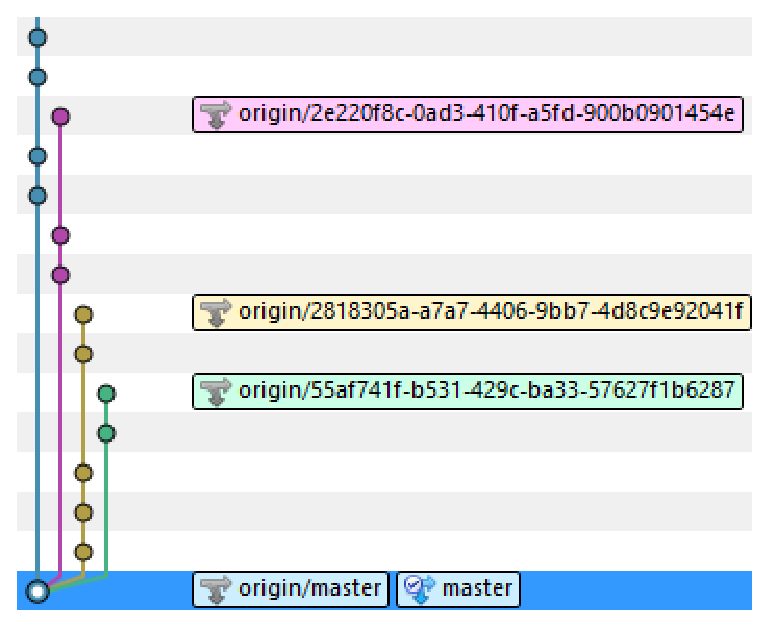
\includegraphics[scale=0.75]{images/tree.eps}
    \caption{Branches du dépôt Git central}
    \label{gitBranch}
\end{center}
\end{figure}

\subsection[Identification des utilisateurs]{Identification des utilisateurs \hyperref[identifPb]{$\uparrow$}}
\label{identifSol}

Le but initial de notre PIDR est de permettre aux professeurs de suivre l'avancement de leurs élèves. Il faut donc pouvoir les identifier sans compromettre leur identité sur le dépôt central. Nous avons donc décider d'utiliser un serveur Play\cite{PlaySite} pour centraliser les données authentifiantes.

\begin{figure}[!h]
\begin{center}
	
\begin{tikzpicture}
\node[server](PC1) at (-3,-1) {};
\node[xshift=-0.8cm,yshift=0.2cm,left of = PC1,align=left](PC1label) {Utilisateur A};

\node(GitA1) at (-5,-2.5) {
\includegraphics[scale=0.25]{images/git.ps}}; 
\node[below of = GitA1,align=left](GitAlabel1) {Git local A1};

\node(GitA2) at (-2,-2.5) {
\includegraphics[scale=0.25]{images/git.ps}}; 
\node[below of = GitA2,align=left](GitAlabel2) {Git local A2};

\node[server](PC2) at (3,-1) {};
\node[xshift=-0.8cm,yshift=0.2cm,left of = PC2,align=left](PC2label) {Utilisateur B};

\node(GitB) at (3,-2.5) {
\includegraphics[scale=0.25]{images/git.ps}}; 
\node[xshift=-0.5cm,left of = GitB,align=left](GitBlabel) {Git local B};
\node[red,inner sep=0mm](croix) at (1.3,0.8) {\begin{LARGE}$\times$\end{LARGE}};

\node[server](PC3) at (4.5,0.5) {};
\node[xshift=0.6cm,right of = PC3,align=left](PC3label) {Utilisateur C};

\node(GitC) at (5.5,-0.5) {
\includegraphics[scale=0.25]{images/git.ps}}; 
\node[xshift=0.7cm,right of = GitC,align=left](GitClabel) {Git local C};


\node[my cloud, minimum width=1.25cm, minimum height=1.55cm,font=\large] (cloud) at (0,2) {Internet};

\node(Git) at (-3.5,3) {
\includegraphics[scale=0.5]{images/git.ps}}; 
\node[xshift=-1cm,left of = Git,align=left](Gitlabel) {Git central};

\node(Play) at (3.5,4) {
\includegraphics[scale=0.15]{images/play.eps}}; 
\node[above of = Play,align=left](Playlabel) {Serveur Play};

\node[server](PCprof) at (6.2,4) {};
\node[xshift=0.8cm,right of = PCprof,align=left](PCproflabel) {Poste professeur};

\draw[thick,darkgray!10!gray] (PC1.north west)--(cloud);
\draw[thick,darkgray!10!gray] (PC1.south east)--(GitA1);
\draw[thick,darkgray!10!gray] (PC1.south west)--(GitA2);
\draw[thick,darkgray!10!gray] (PC2.north east)--(1.3,0.8);
\draw[thick,darkgray!10!gray] (PC2.south)--(GitB);
\draw[thick,darkgray!10!gray] (PC3.north east)--(cloud);
\draw[thick,darkgray!10!gray] (PC3.south)--(GitC);
\draw[thick,darkgray!10!gray] (Git.east)--(cloud);
\draw[thick,darkgray!10!gray] (Play.south west)--(cloud);
\draw[thick,darkgray!10!gray] (Play.east)--(PCprof);
\path[->, red,line width = 0.5mm] (Git)  edge   [bend left=-20]   node {} (Play);
\path[<->, blue,line width = 0.5mm] (GitA2)  edge   [bend left=-80]   node {} (Git.east);
\path[->, darkgray!90,line width = 0.5mm] (PC3) edge [bend left=70] node{} (Play.south west);

\path[<->, blue,line width = 0.5mm] (-4.5,-5)  edge [auto]  node {Git push/pull} (-2,-5);
\path[->, red,line width = 0.5mm] (0,-5)  edge [auto]  node {Git pull} (2.5,-5);
\path[->, darkgray!90,line width = 0.5mm] (4.5,-5)  edge [auto]  node {Liaison d'identité} (7,-5);
\end{tikzpicture}

    \caption{Schéma global}
    \label{schemaGlobal}
\end{center}
\end{figure}


Les élèves seront invités par leur professeur à se connecter sur un serveur Play. Ils devront alors renseigner leur nom, prénom, adresse mail et classe par exemple.

Cela permet de s'assurer que chaque utilisateur \og anonyme\fg{} créé au lancement de la PLM le restera jusqu'au moment où l'utilisateur voudra lier son identité réelle à son identité anonyme. Ce lien se fera sous la forme d'une requête au serveur qui stockera dans une base de données le nom réel, l'adresse mail et le hashé de l'UUID fourni par l'utilisateur afin de savoir à quel utilisateur appartient telle branche vu qu'il n'y a pas d'informations personnelles stockées sur le dépôt distant.

Le reste du PIDR nous ayant déjà demandé beaucoup de temps, le serveur Play ne se trouve pas dans un état très avancé à la fin du projet et ne permet que de pull le dépôt Git central et de consulter la base de données des utilisateurs ayant lié leur identité. Cela pose néanmoins les bases de ce qu'il sera possible de réaliser à l'avenir, comme par exemple offrir aux professeurs une interface web permettant de gérer leurs groupes d'élèves par matière. Voir la figure~\ref{schemaGlobal}.



%
%* solution(s) proposée(s)
%
%* critères de choix
\newpage
\section{Conclusion}

Nous espérons que les modifications que nous avons apporté à la PLM permettront à terme aux professeurs de mieux cerner les besoins et les difficultés de leurs élèves et aux utilisateurs de pouvoir mieux visualiser leurs progrès grâce à la gestion de versions apportée par l'utilisation de Git comme moyen de stockage privilégié. Nous pensons avoir réussi à faire en sorte que la PLM soit bien préparée à se voir ajouter de nouvelles fonctionnalités destinées aux professeurs. Le chemin reste cependant encore long avant un usage efficace de la PLM par ces derniers. Les données collectées seront utilisables non seulement par les professeurs à partir du moment où elles sont authentifiables mais également par les chercheurs puisqu'elles seront anonymes et accessibles à tous. Une perspective directement envisageable qui serait la suite directe de notre travail serait de traiter toutes ces données pour en tirer des représentations graphiques plus facilement interprétables. Dans le cadre des cours à Telecom Nancy, le traitement pourrait être réalisé par le serveur Play, ce qui fournirait aux professeurs une interface graphique agréable à utiliser pour suivre les progrès des élèves. Nous aurions aimé pouvoir réaliser nous-même cette étape si nous n'avions pas été pris par le temps vers la fin du PIDR. Néanmoins, nous pensons avoir laissé une base stable à nos éventuels successeurs pour réaliser ces améliorations et porter encore plus loin la PLM dans son objectif d'enseignement pédagogique de la programmation.


%* résultats actuels
%
%* limites et/ou perspectives

\newpage

\begin{flushleft}
\printbibliography
\end{flushleft}

\listoffigures  % table des figures
\end{document}